t%!TEX root = Simulation.tex

\chapter{Cellular Automata - Chapter 7}

\section{Problem: Slides 1}
\textbf{ Modify the heat flow example to deal with insulated conditions on the top and bottom boundary. Insulation means zero flux or u[N][j] = u[N-1][j]. This implies that instead of a fixed valued ghost points on the top and bottom, you modify the CA rule using the previous relation. }\\
\newline
Cellular automata can be used to study some types of dynamics. In this case, a box with insulated top and bottom walls, and a parabolic heat source on the right wall is presented. The insulated conditions means that the top and bottom boundaries are equal to the grid square below and above them. Using the four neighbors rule, the simplified equation ~\ref{heatDiscrete} is applied to $N-2$ by $N-2$ squares.

Figure ~\ref{heatFlow} shows a grid of 25 x 25 on the left and a grid of 100 x 100 on the right. With the finer grid, a much smoother gradient appears than when using the courser grid. Additionally, the left grid spreads nearly to the left edge before it cools where as the right grid cools approximently halfway across the grid. 

\begin{figure}[tbh]
\begin{center}
	\begin{subfigure}[tbh]{0.47\textwidth}
	\begin{center}
	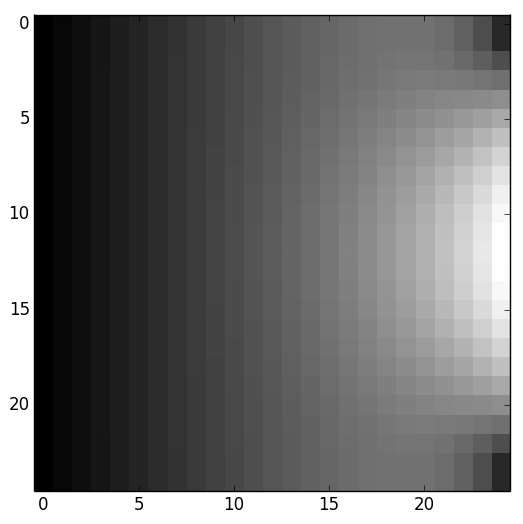
\includegraphics[width=\textwidth]{heatflow/25x25grid10temp.png}
	\caption{ 25 x 25 grid, Temperature = 10 }
	\end{center}
	\end{subfigure}
\hfill
	\begin{subfigure}[tbh]{0.47\textwidth}
	\begin{center}
	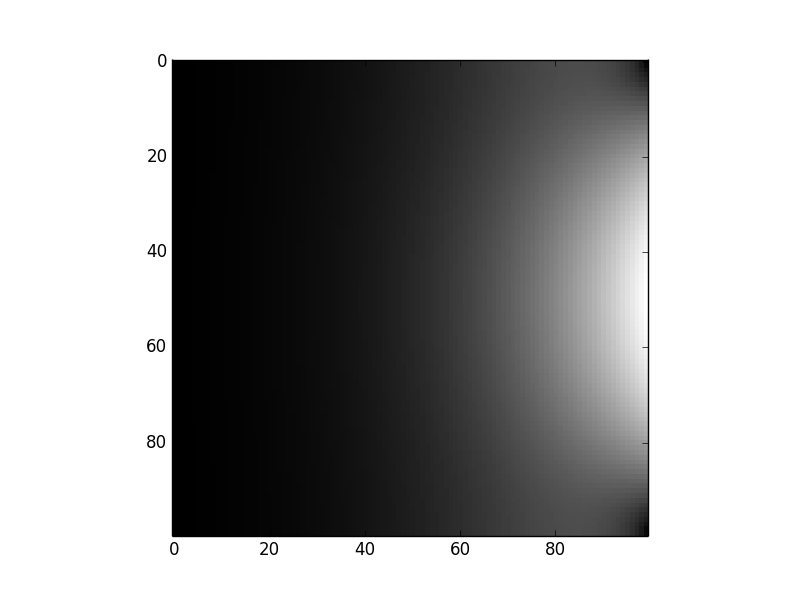
\includegraphics[width=\textwidth]{heatflow/100x100grid10temp.png}
	\caption{ 100 x 100 grid, Temperature = 10 }
	\end{center}
	\end{subfigure}
\hfill
\caption{ Example Heat Flow Grids } \label{heatFlow}
\end{center}
\end{figure}

\begin{equation}
c_{i,j}(t+1) = ( c_{i-1,j}(t) + c_{i+1,j}(t) + c_{i,j-1}(t) + c_{i,j+1}(t)) / 4
\end{equation} \label{heatDiscrete}

\section{Problem: Slides 2}
\textbf{ Reproduce patterns theta, lambda, mu, alpha in the Gray-Scott Model (CA). You don't need to follow their color scheme. } \\
\newline
The Gray-Scott model is used to model pattern formation. The general idea is there's a steady-state grid of some chemical, let's call it $u$. Then, it is perturbed with noise and in the middle with a second chemical, call this one $v$, which reacts with the first chemical. With time, the chemicals reach a steady-state again and a pattern emerges. In equations ~\ref{eqn-grayScott1} and ~\ref{eqn-grayScott2}, $u$ and $v$ are the chemicals reacting, $F$ and $k$ are tuneable parameters which will produce different patterns. Typical values are $ 0.00 < F < 0.08 $ and $ 0.03 < k < 0.07 $ and Figure ~\ref{grayScott-chart} shows values that produce various named patterns.\\

  Using Dr. McGough's code provided on his class website (http://www.mcs.sdsmt.edu/jmcgough/csc492/) and changing the $F$ and $k$ parameters, the images in Figure ~\ref{grayscott-produced} were created. Patterns $\alpha$, $\theta$, and  $\lambda$ are very similar to the examples given in the lecture slides. However, pattern $\mu$ does not compare well to the example. Potential sources of error are gize size, grid granuality or an incorrectly estimated value.

\begin{equation}
\frac{ \partial u}{ \partial t } = d_1  \Delta u - uv^2 + F(1-u)
\end{equation} \label{eqn-grayScott1}

\begin{equation}
\frac{ \partial v}{ \partial t } = d_2 \Delta v + uv^2 - (F+k)v
\end{equation} \label{eqn-grayScott2}

\begin{figure}[tbh]
\begin{center}
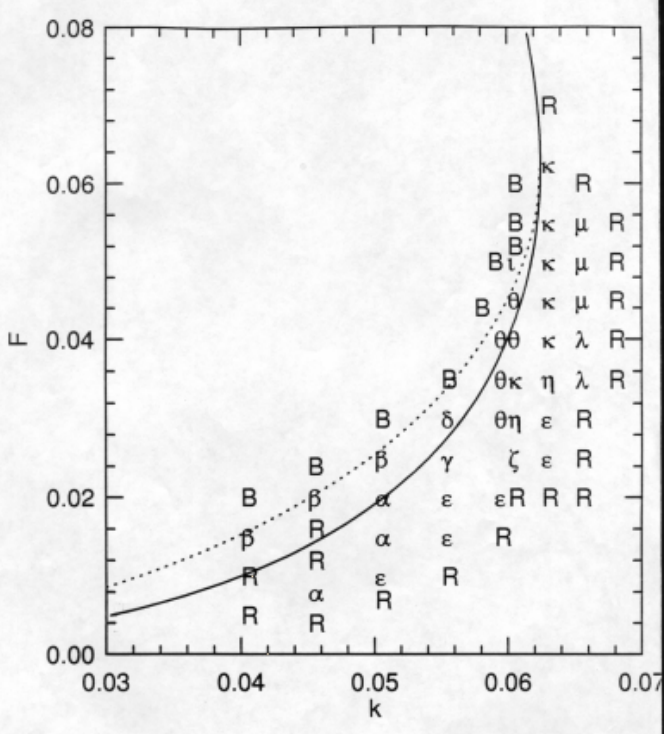
\includegraphics[width=0.47\textwidth]{grayscott/grayscott_chart.png}
\caption{ Gray-Scott Chart }
\end{center}
\end{figure}\label{grayScott-chart}

\begin{figure}[tbh]
\begin{center}
	\begin{subfigure}[tbh]{0.475\textwidth}
	\begin{center}
	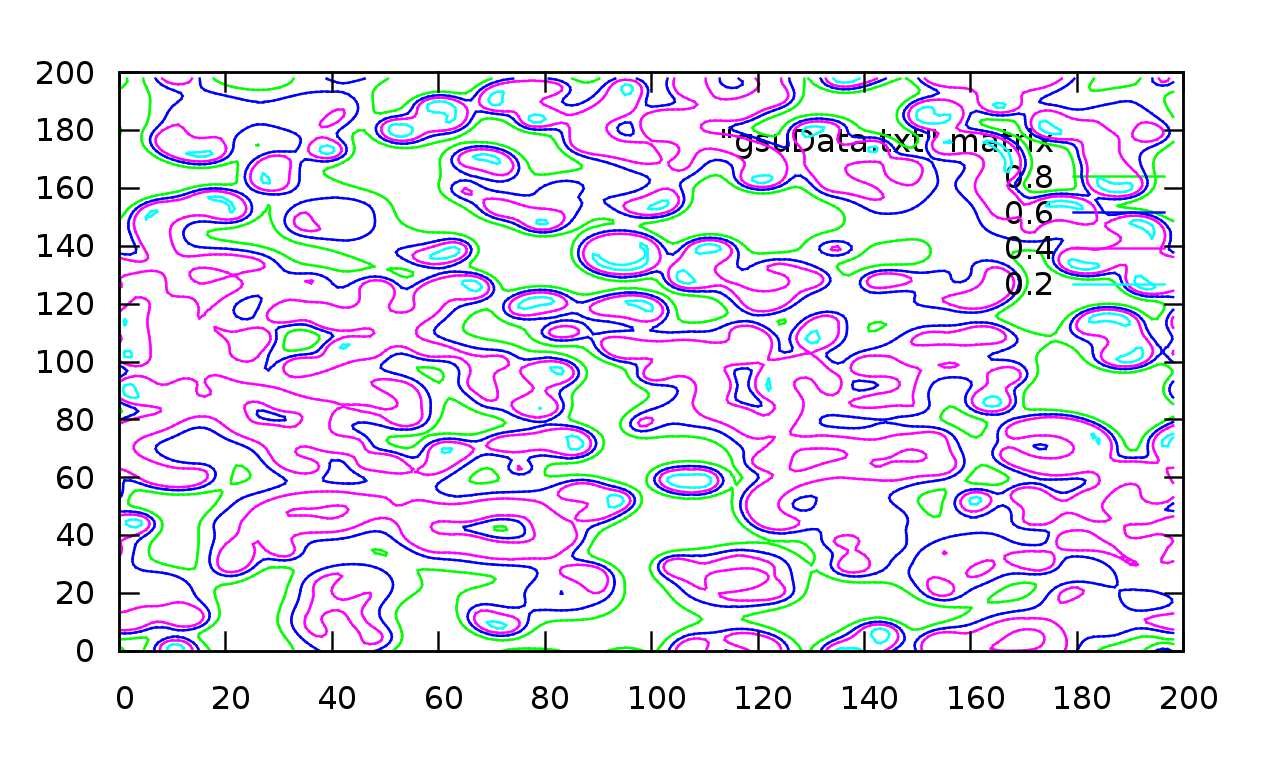
\includegraphics[width=\textwidth]{grayscott/grayscott_alpha.png}
	\caption{ pattern $\alpha$ }
	\end{center}
	\end{subfigure}
\hfill
	\begin{subfigure}[tbh]{0.475\textwidth}
	\begin{center}
	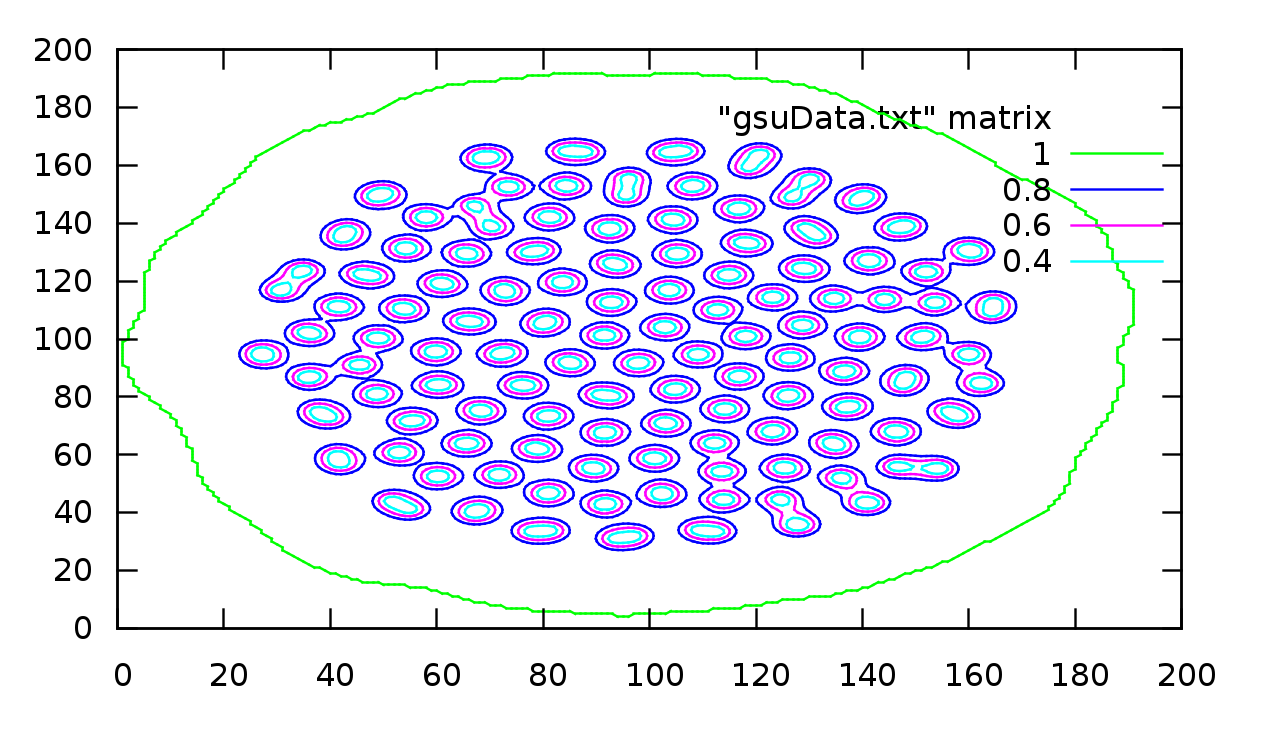
\includegraphics[width=\textwidth]{grayscott/grayscott_lambda.png}
	\caption{ pattern $\lambda$ }
	\end{center}
	\end{subfigure}
\hfill
	\begin{subfigure}[tbh]{0.475\textwidth}
	\begin{center}
	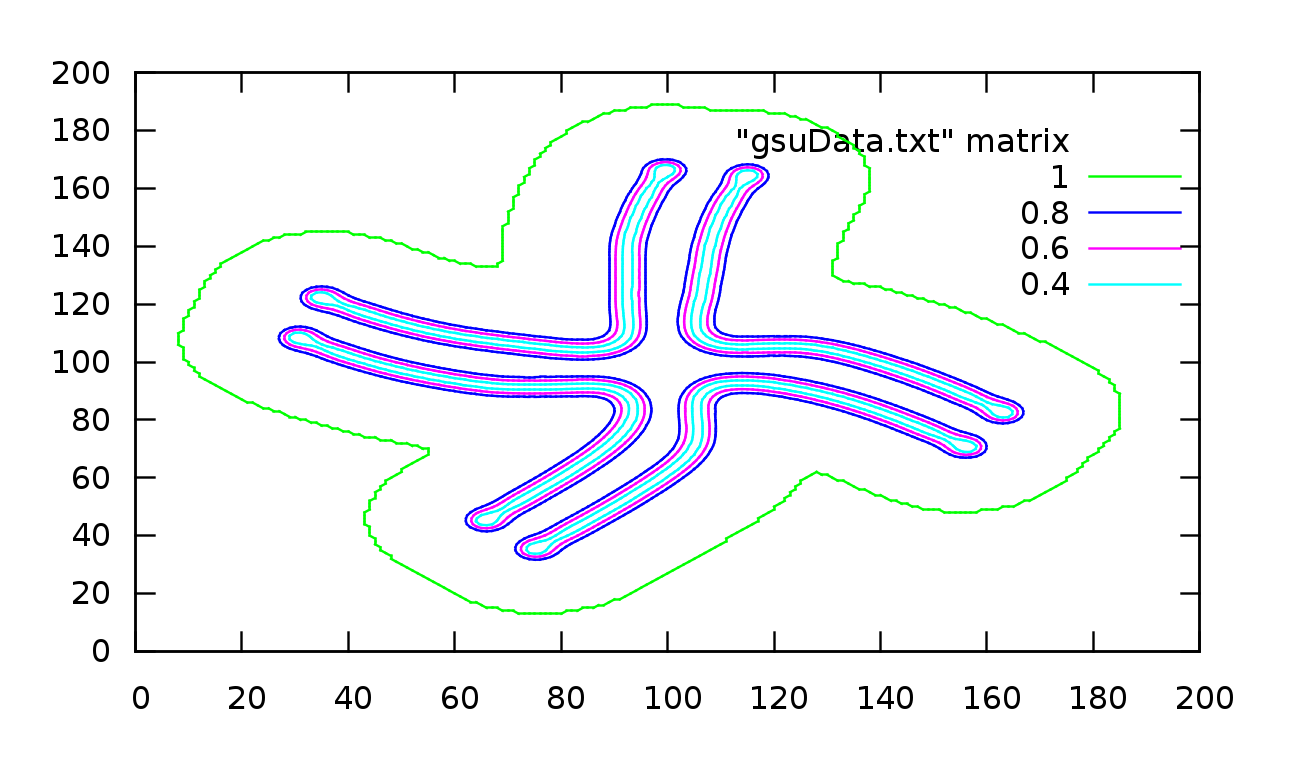
\includegraphics[width=\textwidth]{grayscott/grayscott_mu.png}
	\caption{ pattern $\mu$ }
	\end{center}
	\end{subfigure}
\hfill
	\begin{subfigure}[tbh]{0.475\textwidth}
	\begin{center}
	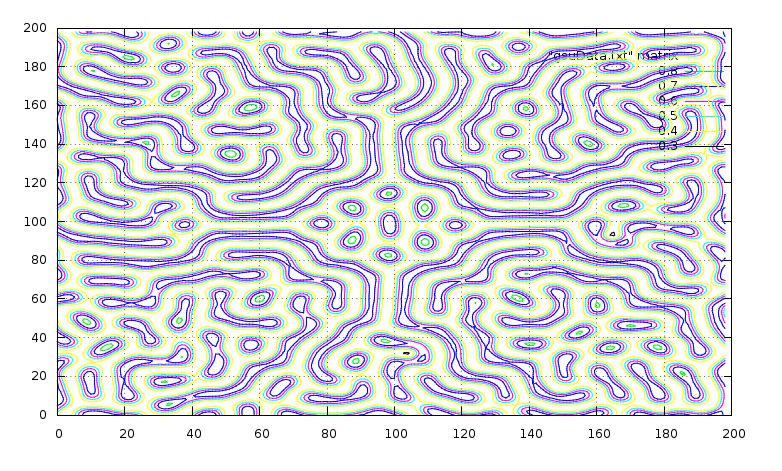
\includegraphics[width=\textwidth]{grayscott/grayscott_theta.png}
	\caption{ pattern $\theta$ }
	\end{center}
	\end{subfigure}
\hfill

\end{center}
\caption{Various Gray-Scott Patterns \label{grayscott-produced} }
\end{figure}